The Ising model provides a simple description of a magnet, stating that in a lattice in $d$ spatial dimension containing $N$ sites, each site is occupied by a state with a magnetic moment (spin). The spins, $s_i$, take the value +1 or -1. This collection of spins has Hamiltonian $\mathcal{H}=-B\sum_i s_i- J\sum_{<ij>}s_is_j$. The first term arises due to the effect of an external magnetic field on the spins, while the second is an interaction term between nearest neighbours. $J>0$ implies that the adjacent spins prefer to be aligned, and the system is a ferromagnet.\\

\noindent In the canonical ensemble, the probability of sitting in a configuration of spins $\{s_i\}$ is given by $p[s_i]=\frac{e^{-\beta E[s_i]}}{Z}$, where $\beta=\frac{1}{T}$ and the normalization factor $Z=\sum_{s_i}e^{-\beta E[s_i]}$ is the partition function.\\ 

\noindent A quantity of interest is the average magnetization $m$, which will play the role of the scalar field later on. It takes values between -1 (low temperature, ordered spins) and +1 (high temperature, random spins). The thermodynamic free energy is defined as $F=-T\log Z$, therefore, if we first sum over all configurations with fixed average magnetisation and subsequently sum over all possible m, we can redefine $Z=\sum_me^{-\beta F(m)}$.

\section{Mean Field Theory}
Since the average magnetization for N lattice sites is $m$, we can construct an average energy of $\frac{E}{N}=-Bm-\frac{1}{2}Jqm^2$, where $q=2d$ is the number of nearest neighbours in $d$ dimensions. A configuration with $N_\uparrow$ up spins and $N_\downarrow=N-N_\uparrow$ down spins has magnetization $m=\frac{2N_\uparrow-N}{N}$ and the number of such configurations is given by $\Omega=\frac{N!}{(N_\uparrow!)(N-N_\uparrow)!}$. Using Stirling's approximation, the average free energy is obtained as

$$f(m)\approx -Bm-\frac{1}{2}Jqm^2+T\left(\frac{1}{2}(1+m)\log(1+m)+\frac{1}{2}(1-m)\log(1-m)\right)$$

\noindent When $m$ is small, we can Taylor expand upto

$$f(m)\approx -Bm+\frac{1}{2}(T-Jq)m^2+\frac{1}{12}Tm^4$$

\noindent The critical temperature is $T_c=Jq$. For $B=0$, temperatures above $T_c$ gives a minimum at $m=0$. However, as the temperature is reduced below $T_c$, the minima now lie at $m=\pm m_0$.

\begin{center}
    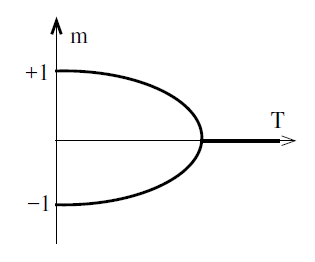
\includegraphics[scale=0.75]{mvsT_B0}
\end{center}

\noindent The magnetization turns off abruptly at the critical temperature, and remains zero for all higher temperatures. This kind of sharp change is characteristic of a second order phase transition.\\

\noindent If $B\neq 0$, we again Taylor expand the free energy and differentiate it. Now, the ground state of the system, i.e. the global minimum of $f(m)$, does not qualitatively change as we vary the temperature. At high temperatures, the magnetisation asymptotes smoothly to zero. Whether the system chooses $m=+1$ or $m=-1$ depends solely on the sign of the magnetic field. There is no phase transition as a function of temperature.

\begin{center}
    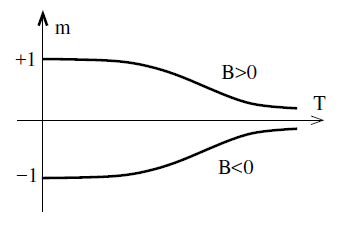
\includegraphics[scale=0.75]{mvsT_B!0}
\end{center}

\noindent Keeping $T$ fixed at a temperature lower than $T_c$, if $B$ is varied continuously such that it changes its sign, the magnetization jumps discontinuously. This is a first order phase transition. For $T>T_c$, any change in $B$ is possible without suffering a phase transition.

\section{Critical Exponents}
The mean field theory is strongly dependent on the dimensionality of the system. For $d=1$, MFT fails completely. Thus the lower critical dimension is 1. There are no phase transitions. For $d=2$ and $d=3$ phase transitions occur, but quantitative predictions around the critical temperature are wrong. For $d>4$, MFT provides correct answers. Thus, the upper critical dimension is 4.\\

$$c=\left[\beta^2\frac{\partial^2}{\partial\beta^2}\log Z\right]_{T\rightarrow T_c}\implies c\sim|T-T_c|^{-\alpha}\hspace{1cm}\alpha=0$$
$$\left[\frac{\partial f}{\partial m}\right]_{B=0}=0\implies m\sim(T-T_c)^\beta\hspace{1cm}\beta=\frac{1}{2}$$
$$\chi=\left[\frac{\partial m}{\partial B}\right]_{T\rightarrow T_c}\implies\chi\sim\frac{1}{|T-T_c|^\gamma}\hspace{1cm}\gamma=1$$
$$\left[\frac{\partial f}{\partial m}\right]_{T=T_c}=0\implies m\sim B^\frac{1}{\delta}\hspace{1cm}\delta=3$$\\

\noindent The coefficients $\alpha$, $\beta$, $\gamma$ and $\delta$ are known as critical exponents. In $d=3$, the Ising model cannot be solved analytically. The numerical values obtained are $\alpha=0.1101$, $\beta=0.2364$, $\gamma=1.2371$ and $\delta=4.7898$.

\noindent The phase transitions for liquid-gas transformations is similar to the Ising model. Here, the critical point is at $T_c=373\,^\circ C$ and $p_c=218$ atm. Similarly, the criritical exponents can be computed using MFT. Calculating $v_\text{gas}-v_\text{liquid}$ gives us $\beta=\frac{1}{2}$ for constant pressure and $\delta=3$ for constant temperature. Analogous to magnetic susceptibilty is the compressibilty $\kappa$, which gives $\gamma=1$. Again, these values are incorrect for $d=2$ and $d=3$.\\

\noindent This is not a coincidence. For a second order phase transition, the underlying microscopic structure is not important. The fact that many different systems can be decribed by the same physics of critical exponents is called universality. This is largely dictated by the symmetries of the system. 

\section{Landau-Ginzburg Theory}
The previous approach treated magnetization to be a constant. In the Landau-Ginzburg theory, it is promoted to the status of a field as its spatial variations are taken into account. The lattice is coarse-grained into boxes of side $a$ and $N'$ sites, each with magnetization $m(\boldsymbol{x})$. As per the definition of a field, $m(\boldsymbol{x})$ is treated to be continuous. Thus, the partition function now becomes an integral over all field configurations, $Z=\int \mathcal{D}m(\boldsymbol{x})\,e^{-\beta F[m(\boldsymbol{x})]}$. The free energy becomes a functional, and mimics the behaviour of the previously studied $\phi^4$ theory, just with spacetime derivatives replaced by normal Euclidean gradient operators. If we replace $m$ by $\phi$,

$$F[\phi(\boldsymbol{x})]=\int d^dx\, \left[\frac{1}{2}\alpha_2 \phi^2+\frac{1}{4}\alpha_4 \phi^4+\frac{1}{2}\gamma(\nabla\phi)^2\right]$$

\noindent $\alpha_2$, $\alpha_4$ and $\gamma$ are functions of temperature.\\

\noindent I will first start with the free field expansion, i.e. $\alpha_4=0$. $\alpha_2$ is redefined as $\mu^2=T-T_c$. The quartic term becomes important as $T\rightarrow T_c$ and its effects cannot be ignored, so the results will not hold when $\mu^2\rightarrow 0$.\\

\noindent The Fourier transform of the field $\phi(\boldsymbol{k})=\int d^dx\, e^{-i\boldsymbol{k}\cdot\boldsymbol{x}}\phi(\boldsymbol{x})$. Since the field is real, $\phi^*(\boldsymbol{k})=\phi(\boldsymbol{-k})$.

\begin{align*}
    \begin{split}
        F[\phi(\boldsymbol{k})]&=\frac{1}{2}\int\frac{d^dk_1}{(2\pi)^d}\int\frac{d^dk_2}{(2\pi)^d}\int d^dx\,(-\gamma\boldsymbol{k}_1\cdot\boldsymbol{k}_2+\mu^2)\phi(\boldsymbol{k}_1)\phi(\boldsymbol{k}_2)e^{i(\boldsymbol{k}_1+\boldsymbol{k}_2)\cdot\boldsymbol{x}}\\
        &=\frac{1}{2}\int\frac{d^dk}{(2\pi)^d}\,(-\gamma k^2+\mu^2)\phi(\boldsymbol{k})\phi^*(\boldsymbol{k})
    \end{split}
\end{align*}

\noindent The free energy decomposes into individual modes. The path integral then becomes

$$Z=\prod_k\int d\phi(\boldsymbol{k})\int d\phi^*(\boldsymbol{k})\,e^{-\frac{\beta}{2}\int\frac{d^dk}{(2\pi)^d}\,(\gamma k^2+\mu^2)|\phi(\boldsymbol{k})|^2}$$

The integral is converted to sum in finite volume $V$, and the Gaussian integral is applied for each $\boldsymbol{k}$.

$$Z=\prod_k\sqrt{\frac{2\pi V}{\beta(\gamma k^2+\mu^2)}}$$\\

\noindent The spatial fluctuations around the ground state are captured by the correlation function. Borrowing results from the previous chapter,

$$\left[\frac{1}{\beta^2}\frac{\delta^2\log Z}{\delta B(\boldsymbol{x})\delta B(\boldsymbol{y})}\right]_{B=0}=\langle\phi(\boldsymbol{x})\phi(\boldsymbol{y})\rangle$$
$$Z[B]=e^{-\beta F}e^{\frac{\beta}{2}\int d^dx\int d^dy\,B(\boldsymbol{x})G(\boldsymbol{x}-\boldsymbol{y})B(\boldsymbol{y})}$$\\

\noindent The Green's function is rotationally invariant, so we can put $|\boldsymbol{x}-\boldsymbol{y}|=r$. Introducing the correlation length as $\xi^2=\frac{\gamma}{\mu^2}$, the Green's function can be solved as a function of $r$ using Bessel functions. 

$$G(r)\sim\frac{1}{r^{d-2}}\hspace{1cm}\text{when }r\ll\xi$$
$$G(r)\sim\frac{e^{-\frac{r}{\xi}}}{r^{\frac{d-1}{2}}}\hspace{1cm}\text{when }r\gg\xi$$\\

\noindent It can be inferred that all correlations die off exponentially quickly at distances $r\gg\xi$. In contrast, for $r\ll\xi$ there is a much slower, power-law fall-off. In this sense, $\xi$ provides a characteristic length scale for the fluctuations. In a given thermal ensemble, there wil be patches where the magnetisation is slightly higher, or slightly lower than the average $\langle m\rangle$. The size of these patches will be no larger than $\xi$. Close to the critical point, the system will undergo fluctuations of arbitrarily large size. This is the essence of a second order phase transition.